\documentclass{article}
\let\biconditional\leftrightarrow
\usepackage{tikz}
\usepackage{fixltx2e}
\usepackage{hyperref}
\begin{document}
Problem 1.
A graph of the CSP 
\vspace{10mm}

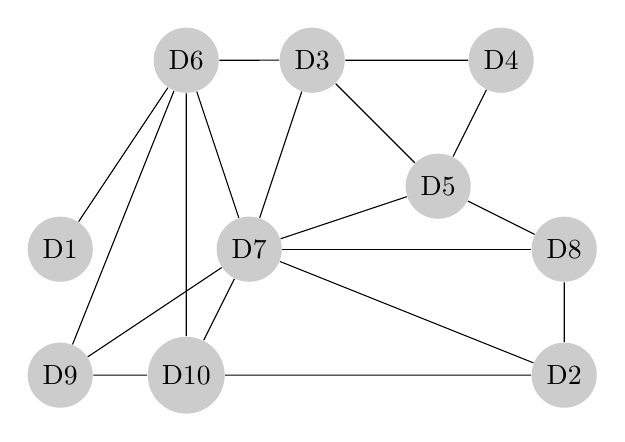
\begin{tikzpicture}
  [scale=.8,auto=left,every node/.style={circle,fill=black!20}]
  \node (n1) at (1,5) {D1};
  \node (n6) at (3,8)  {D6};
  \node (n3) at (5,8)  {D3};
  \node (n7) at (4,5)  {D7};
  \node (n9) at (1,3)  {D9};
  \node (n4) at (8,8)  {D4};
  \node (n5) at (7,6)  {D5};
  \node (n10) at (3,3) {D10};
  \node (n2) at (9,3)  {D2};
  \node (n8) at (9,5)  {D8};
  \foreach \from/\to in {n1/n6,n2/n7,n2/n8,n2/n10,n3/n6,n3/n7,n3/n4,n3/n5,n4/n5,n5/n8,n5/n7,n6/n7,n6/n9,n6/n10,n7/n9,n7/n10,n7/n8,n9/n10}
    \draw (\from) -- (\to);

\end{tikzpicture}
\\
Variables:      Domains\\
D1: District 1 \left\{ {blue, chartreuse, green,red}\right\} \\
D2: District 2 \left\{ {blue, chartreuse, green,red}\right\} \\
D3: District 3 \left\{ {blue, chartreuse, green,red}\right\} \\
D4: District 4 \left\{ {blue, chartreuse, green,red}\right\} \\
D5: District 5 \left\{ {blue, chartreuse, green,red}\right\} \\
D6: District 6 \left\{ {blue, chartreuse, green,red}\right\} \\
D7: District 7 \left\{ {blue, chartreuse, green,red}\right\} \\
D8: District 8 \left\{ {blue, chartreuse, green,red}\right\} \\
D9: District 9 \left\{ {blue, chartreuse, green,red}\right\} \\
D10: District 10 \left\{ {blue, chartreuse, green,red}\right\} \\

\begin{constraints}
Constraints\\
D1\ne D6, D2\ne D7, D2\ne D8, D2\ne D10, D3\ne D6, D3\ne D7, D3\ne D4, \\ D3\ne D5
D4\ne D5, D5\ne D8, D5\ne D7, D6\ne D7, D6\ne D9, D6\ne D10, \\ D7\ne D9, D7\ne D8
D7\ne D10, D9\ne D10 \\
\end{constraints}
\vspace{3mm}

Problem 2
\begin{Problem}

D7 would be chosen since it has 6 constraints which is the most in the constraint problem
D7\ne D2, D7\ne D3, D7\ne D5, D7\ne D6, D7\ne D8, D7\ne D9
\end{Problem}
\vspace{3mm}

Problem 3
Variables:      Domains\\
D1: District 1 \left\{ {blue, chartreuse, green,red}\right\} \\
D2: District 2 \left\{ {blue, chartreuse, green,red}\right\} \\
D3: District 3 \left\{ {blue, chartreuse, green,red}\right\} \\
D4: District 4 \left\{ {blue, chartreuse, green,red}\right\} \\
D5: District 5 \left\{ {blue, chartreuse, green,red}\right\} \\
D6: District 6 \left\{ {blue, chartreuse, green,red}\right\} \\
D7: District 7 \left\{ {blue}\right\} \\
D8: District 8 \left\{ {blue, chartreuse, green,red}\right\} \\
D9: District 9 \left\{ {blue, chartreuse, green,red}\right\} \\
D10: District 10 \left\{ {blue, chartreuse, green,red}\right\} \\
\\

\begin{p3}
Revise(csp,District 2, District 7)\\
District 2 = \left\{ {blue, chartreuse, green,red}\right\} District 7 = \left\{ {blue}\right\} \\
x= blue \\
Check Constraint if x \ne District 7 (false)\\
remove x from District 2 domain \\
District 2 = \left\{ {chartreuse, green,red}\right\} \\
x = chartreuse \\
Check Constraint if x \ne District 7 (true)\\
Keep x in Domain \\
District 2 = \left\{ {chartreuse, green,red}\right\} \\
x = green \\
Check Constraint if x \ne District 7 (true)\\
Keep x in Domain \\
District 2 = \left\{ {chartreuse, green,red}\right\} \\
x = red
Check Constraint if x \ne District 7 (true)\\
Keep x in Domain \\
\end{p3}
\vspace{4mm}

Problem 4
\begin{p4}
District 2 is the next node to consider\\
It is assigned chartreusu because removing any other color will make both \\
neighboring domains 2, so alphabetical choice is made. \\
\end{p4}
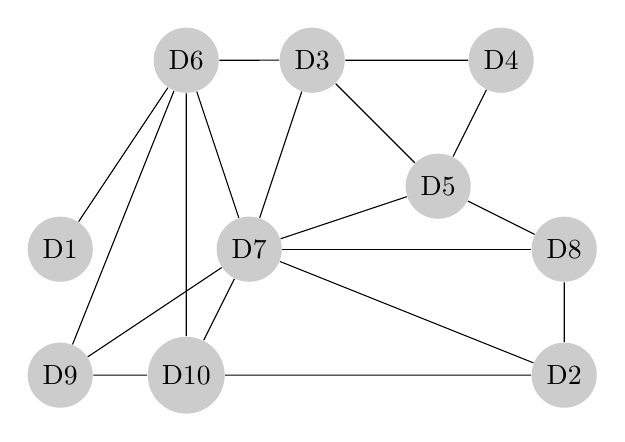
\begin{tikzpicture}
  [scale=.8,auto=left,every node/.style={circle,fill=black!20}]
  \node (n1) at (1,5) {D1};
  \node (n6) at (3,8)  {D6};
  \node (n3) at (5,8)  {D3};
  \node (n7) at (4,5)  {D7};
  \node (n9) at (1,3)  {D9};
  \node (n4) at (8,8)  {D4};
  \node (n5) at (7,6)  {D5};
  \node (n10) at (3,3) {D10};
  \node (n2) at (9,3)  {D2};
  \node (n8) at (9,5)  {D8};
  \foreach \from/\to in {n1/n6,n2/n7,n2/n8,n2/n10,n3/n6,n3/n7,n3/n4,n3/n5,n4/n5,n5/n8,n5/n7,n6/n7,n6/n9,n6/n10,n7/n9,n7/n10,n7/n8,n9/n10}
    \draw (\from) -- (\to);

\end{tikzpicture}
\vspace{3mm} \\
\begin{p42}
Domains\\ 
D1: District 1 \left\{ {blue, chartreuse, green,red}\right\} \\
D2: District 2 \left\{ {chartreuse}\right\} \\
D3: District 3 \left\{ {chartreuse, green,red}\right\} \\
D4: District 4 \left\{ {blue, chartreuse, green,red}\right\} \\
D5: District 5 \left\{ {chartreuse, green,red}\right\} \\
D6: District 6 \left\{ {chartreuse, green,red}\right\} \\
D7: District 7 \left\{ {blue}\right\} \\
D8: District 8 \left\{ {chartreuse, green,red}\right\} \\
D9: District 9 \left\{ {chartreuse, green,red}\right\} \\
D10: District 10 \left\{ {chartreuse, green,red}\right\} \\
\\
Now  After Arc consistency \\
D1: District 1 \left\{ {blue, chartreuse, green,red}\right\} \\
D2: District 2 \left\{ {chartreuse}\right\} \\
D3: District 3 \left\{ {chartreuse, green,red}\right\} \\
D4: District 4 \left\{ {blue, chartreuse, green,red}\right\} \\
D5: District 5 \left\{ {chartreuse, green,red}\right\} \\
D6: District 6 \left\{ {chartreuse, green,red}\right\} \\
D7: District 7 \left\{ {blue}\right\} \\
D8: District 8 \left\{ {green,red}\right\} \\
D9: District 9 \left\{ {chartreuse, green,red}\right\} \\
D10: District 10 \left\{ {green,red}\right\} \\
\end{p42}
chartreuse is removed as domain value from neighbors of D2 \\

\vspace{5mm}

\begin{p5}
Problem 5 \\

1. D8 is next pick green\\
	Thus D2 domain is \left\{ {chartreuse,red}\right\} \\

2. D5 is selected as chartreuse \\
   D3 domain is \left\{ {green,red}\right\} \\

3. D3 is selected as green \\
   D4 domain is \left\{ {blue,red}\right\} \\

4. D4 is selected as blue \\

5. D6 is selected as chartreuse \\
   D1 domain is \left\{{blue,red}\right\} \\
	D9 domain is \left\{{green,red}\right\} \\

6. D9 is selected as green \\
   D10 domain is \left\{ {red}\right\} \\

7. D10 is selected as red \\
   D1 domain is \left\{ {blue}\right\} \\

8. D1 is set to blue
\end{p5}
Final Graph and Domains is \\
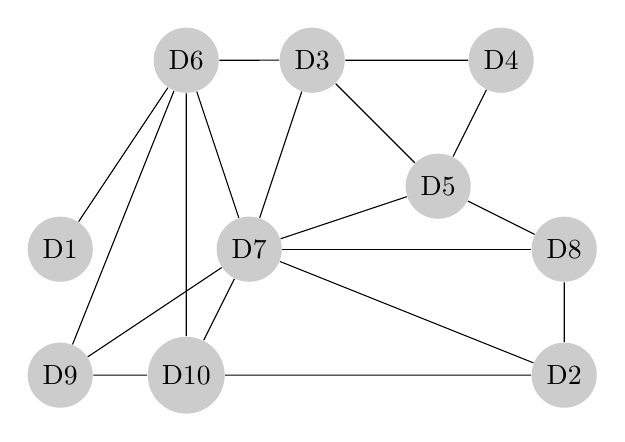
\begin{tikzpicture}
  [scale=.8,auto=left,every node/.style={circle,fill=black!20}]
  \node (n1) at (1,5) {D1};
  \node (n6) at (3,8)  {D6};
  \node (n3) at (5,8)  {D3};
  \node (n7) at (4,5)  {D7};
  \node (n9) at (1,3)  {D9};
  \node (n4) at (8,8)  {D4};
  \node (n5) at (7,6)  {D5};
  \node (n10) at (3,3) {D10};
  \node (n2) at (9,3)  {D2};
  \node (n8) at (9,5)  {D8};
  \foreach \from/\to in {n1/n6,n2/n7,n2/n8,n2/n10,n3/n6,n3/n7,n3/n4,n3/n5,n4/n5,n5/n8,n5/n7,n6/n7,n6/n9,n6/n10,n7/n9,n7/n10,n7/n8,n9/n10}
    \draw (\from) -- (\to);

\end{tikzpicture}
\\
D1: District 1 \left\{ {blue}\right\} \\
D2: District 2 \left\{ {chartreuse}\right\} \\
D3: District 3 \left\{ {green}\right\} \\
D4: District 4 \left\{ {blue}\right\} \\
D5: District 5 \left\{ {chartreuse}\right\} \\
D6: District 6 \left\{ {chartreuse}\right\} \\
D7: District 7 \left\{ {blue}\right\} \\
D8: District 8 \left\{ {green}\right\} \\
D9: District 9 \left\{ {green}\right\} \\
D10: District 10 \left\{ {red}\right\} \\

If we didn't use forward checking we would end up in a fail state more often because we
chose a new state without considering the future possible conflicts (consequences)
\\
\\
\\
Problem 6 \\
Steps: \\
Bicondition elimination \\
Implication elimation \\
Distributive properties \\
\\
\begin{p6}
1. W\textsubscript{3,3} \biconditional \big(S\textsubscript{2,3} \land S\textsubscript{3,2} \land S\textsubscript{3,4} \land S\textsubscript{4,3} \big)\\
\\
2. W\textsubscript{3,3} \to \big(S\textsubscript{2,3} \land S\textsubscript{3,2} \land S\textsubscript{3,4} \land S\textsubscript{4,3} ) \land (S\textsubscript{2,3} \land S\textsubscript{3,2} \land S\textsubscript{3,4} \land S\textsubscript{4,3} \big) \to W\textsubscript{3,3} \\
\\
3. \big[ \neg W\textsubscript{3,3} \lor \big(S\textsubscript{2,3} \land S\textsubscript{3,2} \land S\textsubscript{3,4} \land S\textsubscript{4,3}\big) \big] \land \big[ \neg \big(S\textsubscript{2,3} \land S\textsubscript{3,2} \land S\textsubscript{3,4} \land S\textsubscript{4,3}\big) \lor W\textsubscript{3,3} \big] \\
\\
4. \big[ \neg W\textsubscript{3,3} \lor \big(S\textsubscript{2,3} \land S\textsubscript{3,2} \land S\textsubscript{3,4} \land S\textsubscript{4,3}\big) \big] \land \big[\big(\neg S\textsubscript{2,3} \land \neg S\textsubscript{3,2} \land \neg S\textsubscript{3,4} \land \neg S\textsubscript{4,3}\big) \lor W\textsubscript{3,3} \big] \\
\\
5. \big(\neg W\textsubscript{3,3} \lor S\textsubscript{2,3} \big) \land \big(\neg W\textsubscript{3,3} \lor S\textsubscript{3,2}\big) \land \big(\neg W\textsubscript{3,3} \lor S\textsubscript{3,4}\big) \land  \big(\neg W\textsubscript{3,3} \lor S\textsubscript{4,3} \big) \\ \land( \neg S\textsubscript{2,3} \lor \neg S\textsubscript{3,2} \lor \neg S\textsubscript{3,4} \lor \neg S\textsubscript{4,3} \lor W\textsubscript{3,3} \big) \\
\end{p6}
\\
\\
Transcript \\
\\
\begin{verbatim}
to_cnf("W33 <=> S23 & S32 & S34 & S43")

>>((W33 | ~S23) & (S23 | ~W33) & S32 & S34 & S43)

to_cnf("(~W33 | S23)&(~W33| S32)&(~W33| S34)&(~W33| S43)& (~S23| ~S32| ~S34| ~S43 | W33)")

>>((~W33 | S23) & (~W33 | S32) & (~W33 | S34) & (~W33 | S43) & 
(~S23 | ~S32 | ~S34 | ~S43 | W33)
\end{verbatim}


\end{document}















